% Created 2023-09-07 Thu 13:40
% Intended LaTeX compiler: pdflatex
\documentclass[11pt]{article}
\usepackage[utf8]{inputenc}
\usepackage[T1]{fontenc}
\usepackage{graphicx}
\usepackage{longtable}
\usepackage{wrapfig}
\usepackage{rotating}
\usepackage[normalem]{ulem}
\usepackage{amsmath}
\usepackage{amssymb}
\usepackage{capt-of}
\usepackage{hyperref}
\usepackage{siunitx, graphicx}
\graphicspath{ {./images/} }
\author{Hankertrix}
\date{\today}
\title{Cells Cheat Sheet}
\hypersetup{
 pdfauthor={Hankertrix},
 pdftitle={Cells Cheat Sheet},
 pdfkeywords={},
 pdfsubject={},
 pdfcreator={Emacs 29.1 (Org mode 9.6.6)}, 
 pdflang={English}}
\begin{document}

\maketitle
\setcounter{tocdepth}{2}
\tableofcontents

\newpage

\section{Definitions}
\label{sec:org2bdd88a}

\subsection{Unicellular organisms}
\label{sec:orgc88e936}
A unicellular organism is an organism that consists of only a single cell that does everything. Prokaryotes and protists come under this category. The word "prokaryotes" means "before nucleus" in Greek, indicating that they do not have a nucleus. All organisms in the domain Bacteria and Archaea are prokaryotes. We sometimes refer to them as eubacteria and archaeabacteria. The word "eukaryotes", on the other hand, means "true nucleus" in Greek, and protists belong to this category. Almost all eukaryotes besides protists are multicellular organisms.

\subsection{Multicellular organisms}
\label{sec:org721cf76}
Almost all other eukaryotes besides protists are multicellular organisms. The cells in multicellular organisms developed into specialised types, and this phenomenon is called differentiation. The cells cannot "do-it-all" any more and hence they work together to keep the organism "alive".

\subsection{Resolution}
\label{sec:org87263df}
Resolution refers to the minimum distance that two points can be apart and still be distinguished as two separate points. The limit of resolution of the human eye is only about 100 \(\unit{\micro\metre}\). One way to increase resolution is to increase magnification, such as by using a microscope.

\subsection{Compound light microscopes}
\label{sec:org6709044}
Compound light microscopes uses sets of magnifying lenses to resolve structures that are separated by more than 200 \(\unit{\nano\metre}\).

\subsection{Electron microscopes}
\label{sec:org4d00f9b}
Electron microscopes have 1000 times the resolving power of light microscopes and can resolve objects as close as 0.2 \(\unit{\nano\metre}\) apart.

\newpage

\subsection{Plasma membrane}
\label{sec:org6335b75}
A plasma membrane is essentially a sheet of lipids with embedded proteins. It is a common feature to all cells, although the chemical composition may differ. It defines the boundary of a cell. The lipid bilayer forms the foundation of the membrane and the molecules that make up the lipid layers are called phospholipids. Some proteins form channels that span the membrane (transmembrane proteins) and other proteins are integrated into the structure of the membrane (cell surface proteins).

\subsection{Diffusion}
\label{sec:orgd8b99ea}
Diffusion is when there is net movement of molecules from an area of higher concentration to an area of lower concentration. Molecules diffuse down a concentration gradient from higher to lower concentrations, and diffusion ends when equilibrium is reached. Cells move material in and out of a cell via diffusion.
\\[0pt]

Only certain substances undergo diffusion across the plasma membrane, like molecules such as oxygen, carbon dioxide, and non-polar lipids. Ions and polar molecules cannot cross the interior of the membrane. However, water is able to diffuse freely across the plasma membrane despite being polar thanks to \textbf{aquaporins}.
\\[0pt]

Diffusion causes water molecules to distribute themselves equally on both sides of a semi-permeable membrane. Addition of solute molecules that cannot cross the membrane reduces the number of free water molecules on that side, as they bind to the solute. Diffusion then causes free water molecules to move from the side where water's concentration is higher, to the solute side where its concentration is lower.

\subsection{Osmosis}
\label{sec:orge34fd0a}
Osmosis is the movement of solvent or water from a region of lower solute concentration to a region of higher solute concentration through a semi-permeable membrane.

\subsection{Aquaporins}
\label{sec:org876cb91}
Aquaporins are selective channels that permit water to cross.

\subsection{Osmotic concentration}
\label{sec:org1e25146}
The concentration of all molecules dissolved in a solution is called the osmotic concentration of the solution.

\subsection{Isotonic}
\label{sec:org0c417d1}
Isotonic refers to the situation where the osmotic concentrations of two solutions are equal.

\subsection{Hypertonic}
\label{sec:org02fa183}
If two solutions have unequal osmotic concentration, the solution with the higher solute concentration is said to be hypertonic.

\subsection{Hypotonic}
\label{sec:org664c246}
If two solutions have unequal osmotic concentration, the solution with the lower solute concentration is said to be hypotonic.

\subsection{Osmotic pressure}
\label{sec:org2d384c6}
Osmotic pressure is the pressure caused by the movement of water into a cell.

\subsection{Endocytosis}
\label{sec:org7dada5b}
Endocytosis is the engulfing of substances outside the cell to form a vesicle that is brought inside the cell. This is achieved through the folding of membranes.

\subsection{Exocytosis}
\label{sec:orgb1a9441}
Exocytosis is the discharge of substances from vesicles at the inner surface of the cell. This is achieved through the folding of membranes.

\newpage

\subsection{Selective permeability}
\label{sec:org242ba8e}
\begin{itemize}
\item Allows cells to control specifically what enters and leaves.
\item Involves using proteins in the membrane for transporting substances across.
\item Transport can be down a concentration gradient or against a concentration gradient.
\end{itemize}

\subsection{Selective diffusion}
\label{sec:org046b474}
\begin{itemize}
\item Proteins act as open channels for whatever that is small enough to fit inside the channel.
\item This form of diffusion is common in ion transport.
\end{itemize}

\subsection{Facilitated diffusion}
\label{sec:orgf45f174}
\begin{itemize}
\item Proteins act as carriers that can bind only to specific molecules and transport them.
\item Transport is limited by the availability of carriers.
\item When all carriers are in use, then the transport is saturated.
\end{itemize}

\subsection{Nucleoid region}
\label{sec:org8138535}
Nucleoid region refers to an area of the cell where the DNA is localised.

\subsection{Flagellum (plural: flagella)}
\label{sec:orga92b2f2}
The flagellum is a threadlike structure made of protein fibres that extends from the cell surface that aids in locomotion and feeding. There may be one or many flagella.
\\[0pt]

The flagella of bacteria rotate to generate motion and are made of flagellin, while eukaryotic flagella are made of microtubule beat and do not rotate. The bacterial flagella motor is composed of approximately 35 proteins and has a base and a hook that connects the cell surface to the filament of the flagellum.

\subsection{Pilus (plural: pili)}
\label{sec:org0792a3a}
Pilus is a short appendage that aids in attaching to substrates and in exchanging genetic information between cells.

\subsection{Peptido}
\label{sec:org455c9b5}
Peptido refers to "peptides" with a number of amino acids.

\subsection{Glycan}
\label{sec:org070b5c5}
Glycan refers to complexes composed of sugar units.

\subsection{Nucleus}
\label{sec:org4f97920}
The nucleus is the command and control centre of the cell. It also stores hereditary information. The nuclear surface is bound by a double-membrane called the \textbf{nuclear envelop}. Groups of proteins form openings in the nuclear envelope called \textbf{nuclear pores} that permit proteins and ribonucleic acid (RNA) to pass in and out of the nucleus.
\\[0pt]

The DNA of eukaryotes is packaged into linear chromosomes, and chromosomal DNA is organised into nucleosomes which consist of a portion of DNA wrapped around proteins called histones. When the cell is not dividing, the chromosomes exist as threadlike strands called \textbf{chromatin}. Whether the tails of histones are methylated (\(-CH_3\)) or acetlylated (\(-COCH_3\)) determines whether the chromatin exists as heterochromatin (more densely compacted) or \textbf{euchromatin} (less densely compacted) respectively.

\subsection{Nucleolus}
\label{sec:org1be3cbc}
The nucleolus is a region of the nucleus where ribosomes are assembled.

\subsection{Ribosomes}
\label{sec:org8de0115}
Ribosomes are structures that build up proteins and consist of ribosomal RNA and several different kinds of proteins.

\newpage

\subsection{Endomembrane system}
\label{sec:org93e617e}
The endomembrane system refers to the collection of internal membranes in the cell that make up organelles such as the endoplasmic reticulum, Golgi complex, lysosomes and vacuoles. Some of the membranes form channels and interconnections. Other portions become isolated spaces enclosed by membranes, known as vesicles.

\subsection{Endoplasmic reticulum (ER)}
\label{sec:org6665d04}
Endoplasmic reticulum (ER) is an extensive system of internal membranes. The portion of the endoplasmic reticulum dedicated to protein synthesis is called the \textbf{rough endoplasmic reticulum}. The surface of this region looks pebbly and the rough spots are due to embedded ribosomes.
\\[0pt]

The portion of the endoplasmic reticulum that aids in the manufacture of carbohydrates and lipids is called the smooth endoplasmic reticulum. The surface of this region looks smooth because embedded ribosomes are scarce.

\subsection{Golgi bodies}
\label{sec:org25b386c}
The Golgi bodies are flattened stacks of membranes scattered through the cytoplasm and their numbers vary depending on the cell. Their function is to collect, package and distribute molecules manufactured in the cell, such as the molecules made by the endoplasmic reticulum.

\subsection{Golgi complex}
\label{sec:orgc117996}
The Golgi complex refers to the collection of Golgi bodies in the cell. The endoplasmic reticulum and the Golgi complex function together as a transport system of synthesised macromolecules in the cell.

\subsection{Lysosomes}
\label{sec:org8d1aa84}
The lysosomes are membrane-bound structures that contain enzymes that the cell uses to break down macromolecules. The worn-out parts of the cell are broken down and their components are recycled to form new parts. The particles that the cell has ingested are also digested by the lysosomes.

\subsection{Vacuoles}
\label{sec:orgd0b5e78}
Vacuoles are membrane-bound storage compartments. In plants, the \textbf{central vacuole} stores water and dissolved substances and in some protists, the \textbf{contractile vacuole} is found near the cell surface of some protists and accumulates excess water from inside the cell that it then pumps out.

\subsection{Mitochondria}
\label{sec:org1e66a2a}
Mitochondria are cellular powerhouses. They are the sites for chemical reactions called \textbf{oxidative metabolism} and the organelle is surrounded by two membranes, the inner and outer membrane. Mitochondria also contain their own molecule of circular DNA, but they cannot be grown free of the cell and are totally dependent on the cells within which they occur.

\subsection{Chloroplasts}
\label{sec:orgd1d2e60}
Chloroplasts are the sites of \textbf{photosynthesis}, which are only found in photosynthetic organisms such as plants. The organelle is also surrounded by two membranes, the inner and outer membrane. Chloroplasts also contain their own molecule of circular DNA, but they cannot be grown free of the cell and are totally dependent on the cells within which they occur.

\subsection{Endosymbiosis}
\label{sec:org4460e69}
Endosymbiosis is a theory that states that some organelles evolved from a symbiosis in which one cell of a prokaryotic species was engulfed by and lived inside a cell of another species of prokaryote (that was a precursor to eukaryotes). The engulfed species provided their own hosts with advantages because of special metabolic activities. The modern organelles of mitochondria and chloroplasts are believed to have evolved from these endosymbiotic prokaryotes.

\newpage

\subsection{Cytoskeleton}
\label{sec:org7f23bf2}
The cytoskeleton comprises an internal framework of protein fibres that anchors organelles to fixed locations, supports the shape of the cell, and helps organise ribosomes and enzymes needed for synthesis.
\\[0pt]

The cytoskeleton is made of three different types of protein fibres:
\begin{itemize}
\item Intermediate filaments, which are thick ropes of intertwined protein
\item Microtubules, which are hollow tubes made up of the protein tubulin
\item Microfilaments, which are long, slender microfilaments made of the protein actin
\end{itemize}

\subsection{Centrioles}
\label{sec:orgbc1a96f}
Centrioles are complex structures that assemble microtubules in animal cells and the cells of most protists. They occur in pairs and are found near the nuclear envelop. They are also composed of microtubules.

\subsection{Cellular motion}
\label{sec:orga80070d}
Cellular motion is associated with the movement of actin microfilaments or microtubules. Some cells "crawl" by coordinating the rearrangement of actin microfilaments and some cells "swim" by coordinating the beating of microtubules grouped together to form flagella or cilia.

\section{Cell Theory}
\label{sec:orgf00f0ae}
\begin{enumerate}
\item All organisms are composed of one or more cells.
\item Cells are the smallest living things.
\item Cells arise only by division of previously existing cells.
\end{enumerate}

\section{Size of cells}
\label{sec:org1da4227}
Cells are not of the same shapes and sizes, but they are generally small. Larger cells do not work very efficiently. This is why when organisms become bigger, they have to be multicellular instead of simply becoming a larger cell. Many small cells working together is more efficient that having a single enormous cell.

\section{Small vs large cells}
\label{sec:org36ea311}
\begin{itemize}
\item Larger cells are more difficult to control because of the \textbf{longer distance} between the command centre at the core and the peripheral regions, so organisms that comprises many small cells are at an efficiency advantage.
\item Smaller cells also have a greater surface area to volume ratio as the volume increases more rapidly than surface area as the cell size grows. Since a cell's surface provides the interior's only opportunity to interact with the environment, a larger surface area is beneficial to the cell.
\end{itemize}

\newpage

\section{Types of cells}
\label{sec:org76b20e8}

\subsection{Prokaryotic cells}
\label{sec:orgf4143e4}
\begin{itemize}
\item Lack a nucleus
\item Contains a \textbf{plasma membrane} surrounding a cytoplasm without interior compartments.
\item Might have a \textbf{cell wall} that is made of carbohydrates to confer rigid structure.
\item Might have a \textbf{capsule} that may surround the cell wall.
\item The cytoplasm is uniform with little or no internal support framework.
\item Ribosomes (sites for protein synthesis) are scattered throughout the cytoplasm.
\item Nucleoid region is not membrane-bound and is not a true nucleus. In general, genomic DNA is organised as \textbf{circular} chromosomes.
\item Does not have an extensive system of internal membranes.
\item All bacteria and archaea have this cell type.
\end{itemize}

\subsubsection{Bacteria domain}
\label{sec:orgeb8f142}
\begin{itemize}
\item 1 - 10 \(\unit{\micro\metre}\)
\item Cell wall made of \textbf{peptidoglycan}
\item Cell membrane based on fatty acids
\item No membrane-bound organelles
\end{itemize}

\newpage

\subsubsection{Archaea domain}
\label{sec:org57a04e9}
\begin{itemize}
\item 1 - 10 \(\unit{\micro\metre}\)
\item Cell wall made of various molecules such as pseudopeptidoglycan and proteins
\item Cell membrane based on non-fatty acids lipids (isoprene)
\item No membrane-bound organelles
\item Live in extreme conditions such as the Dead Sea (unusual salt composition) and deep sea vents (temperatures above 100 \(\unit{\degreeCelsius}\) and pressure above 200 atmospheres)
\end{itemize}

The Dead Sea has a salt concentration of 33\% w/v, composed of 53\% \(MgCl_2\), 37\% \(KCl\), and 8\% \(NaCl\). In contrast, the ocean is mostly \(NaCl\) and only has a salt concentration of 3\% w/v. The human body only has a salt concentration of around 1\% w/v, and it is a mixture of \(MgCl_2\), \(KCl\) and \(NaCl\).
\\[0pt]

The membrane phospholipids in Archaea carry isoprene chains instead of fatty acid chains. The chirality of the central carbon is also different (L-isomer instead of D-isomer). Tetraether membranes are also found in hyperthermophiles, which are archaea.

\newpage

\subsection{Eukaryotic cells}
\label{sec:org9c9a549}
\begin{itemize}
\item 10 - 100 \(\unit{\micro\metre}\)
\item Has a nucleus, which is a membrane-bound compartment for DNA and is also what gives eukaryotes their name
\item Larger and more complex than prokaryotic cells
\item The size range among eukaryotic cells is much wider because of the diversity (from protists like paramecium to different types of cells of plants and animals)
\item Has a plasma membrane encasing the cytoplasm
\item The cytoplasm is semi-fluid and contains a network of protein fibres that form a scaffold called a cytoskeleton
\item Its internal membranes form compartments called organelles
\item Cell wall made of cellulose or chitin in many cases
\item Cell membrane based on fatty acids
\item All organisms other than bacteria or archaea have this cell type
\end{itemize}

\subsubsection{Differences between eukaryotic cells}
\label{sec:org1149c49}
\begin{itemize}
\item The plasma membrane of animal cells contains cholesterol, but plant cells do not
\item The cells of plants, fungi and many protists have a cell wall beyond the plasma membrane
\item All plants and many protists contain organelles called chloroplasts
\item Plants contain a central vacuole
\item Only animal cells contain centrioles
\end{itemize}

\section{Chart of relative sizes}
\label{sec:org8254fd4}
Below is the chart showing the relative sizes of organisms:

\[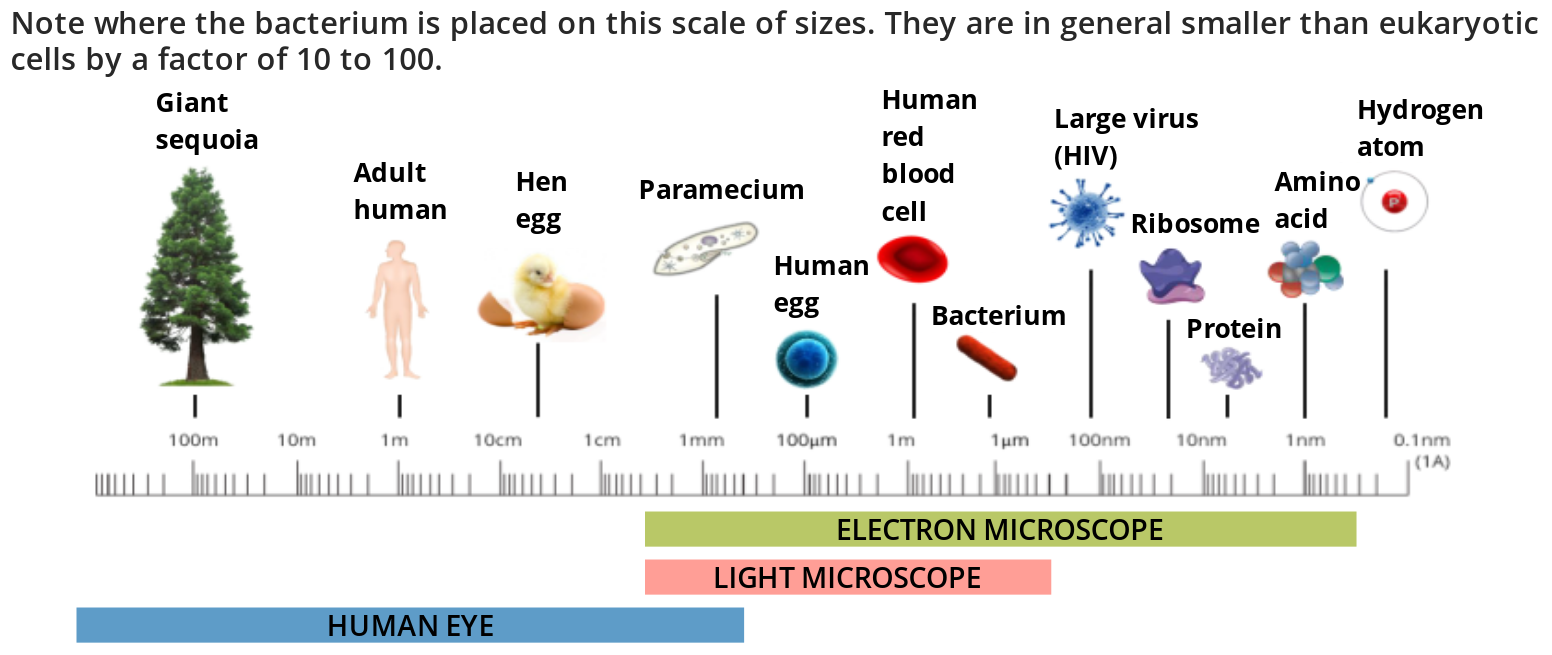
\includegraphics[width = \textwidth]{relative-sizes}\]

\section{DNA packaging}
\label{sec:org216f585}
The \emph{E. coli} chromosome consists of a circular DNA approximately 1 \(\unit{\milli\metre}\), while the bacterium itself is only about 2 \(\unit{\micro\metre}\) long. This means that the DNA has to be packaged and compacted, which is achieved through supercoiling and assistance by a specific set of nucleoid-associated proteins.

\newpage

\section{Types of bacteria}
\label{sec:org5d467d6}
Bacteria can either be Gram-positive or Gram-negative, and it is distinguished by the structures of the cell wall. This can be tested through Gram staining procedure of a bacterial specimen followed by observation under a light microscope.
\\[0pt]

Both types of cell walls carry a peptidoglycan layer.

\subsection{Gram-positive}
\label{sec:orgbae5499}
\begin{itemize}
\item Thicker
\item Stained purple
\end{itemize}

\subsection{Gram-negative}
\label{sec:org011dd32}
\begin{itemize}
\item Has an outer membrane next to the peptidoglycan layer
\item Stained pink
\end{itemize}

\section{Gram stain procedure}
\label{sec:org4a7d13e}
\begin{enumerate}
\item When crystal violet is applied, both types of cells take in the dye.
\item When Gram's iodine is next added, a crystal of violet-iodine complex is formed inside the cells.
\item After an alcohol wash, only the Gram-positive bacteria retain the crystal violet dye in their cells.
\item Afterwards, safarin dye is added and the pink or red colour of the safarin dye is only visible on Gram-negative cells.
\end{enumerate}

\section{Structures}
\label{sec:orgdea8541}

\subsection{Animal cells}
\label{sec:org368f058}
\[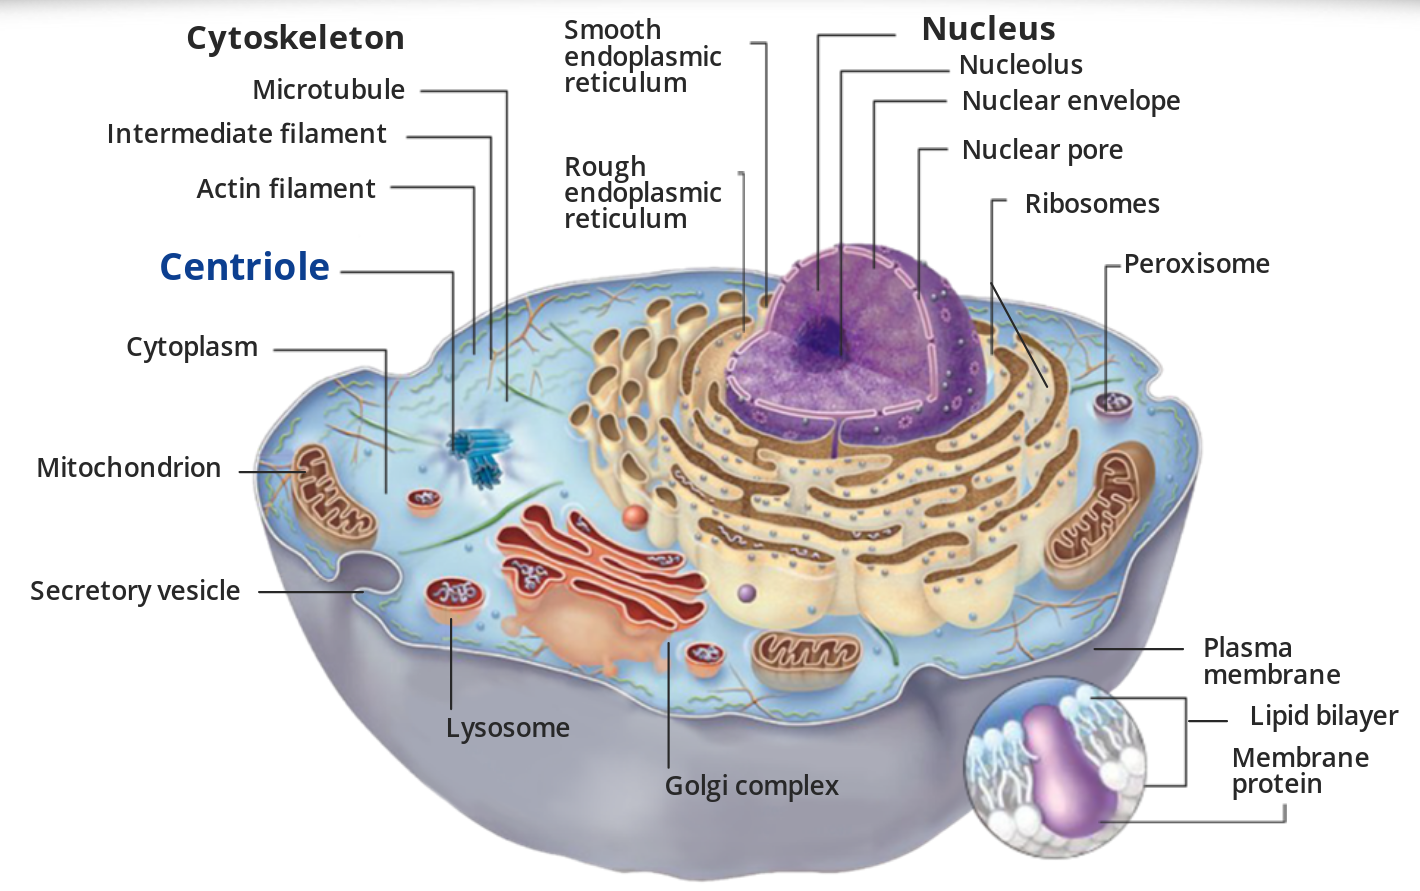
\includegraphics[width = \textwidth]{animal-cell-structure}\]

\subsection{Plant cells}
\label{sec:org1e78dff}
\[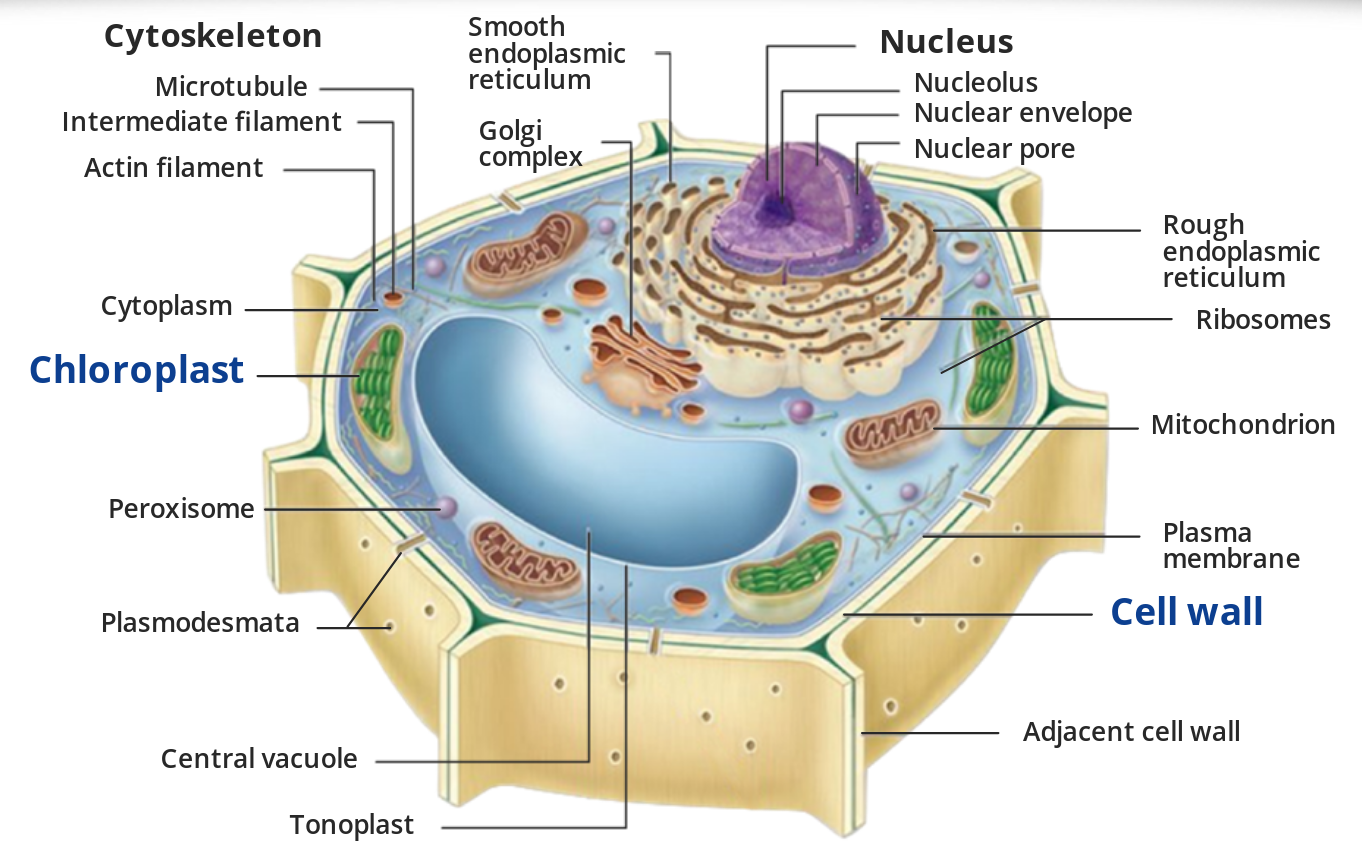
\includegraphics[width = \textwidth]{plant-cell-structure}\]

\subsection{Nucleus}
\label{sec:orge605331}
\[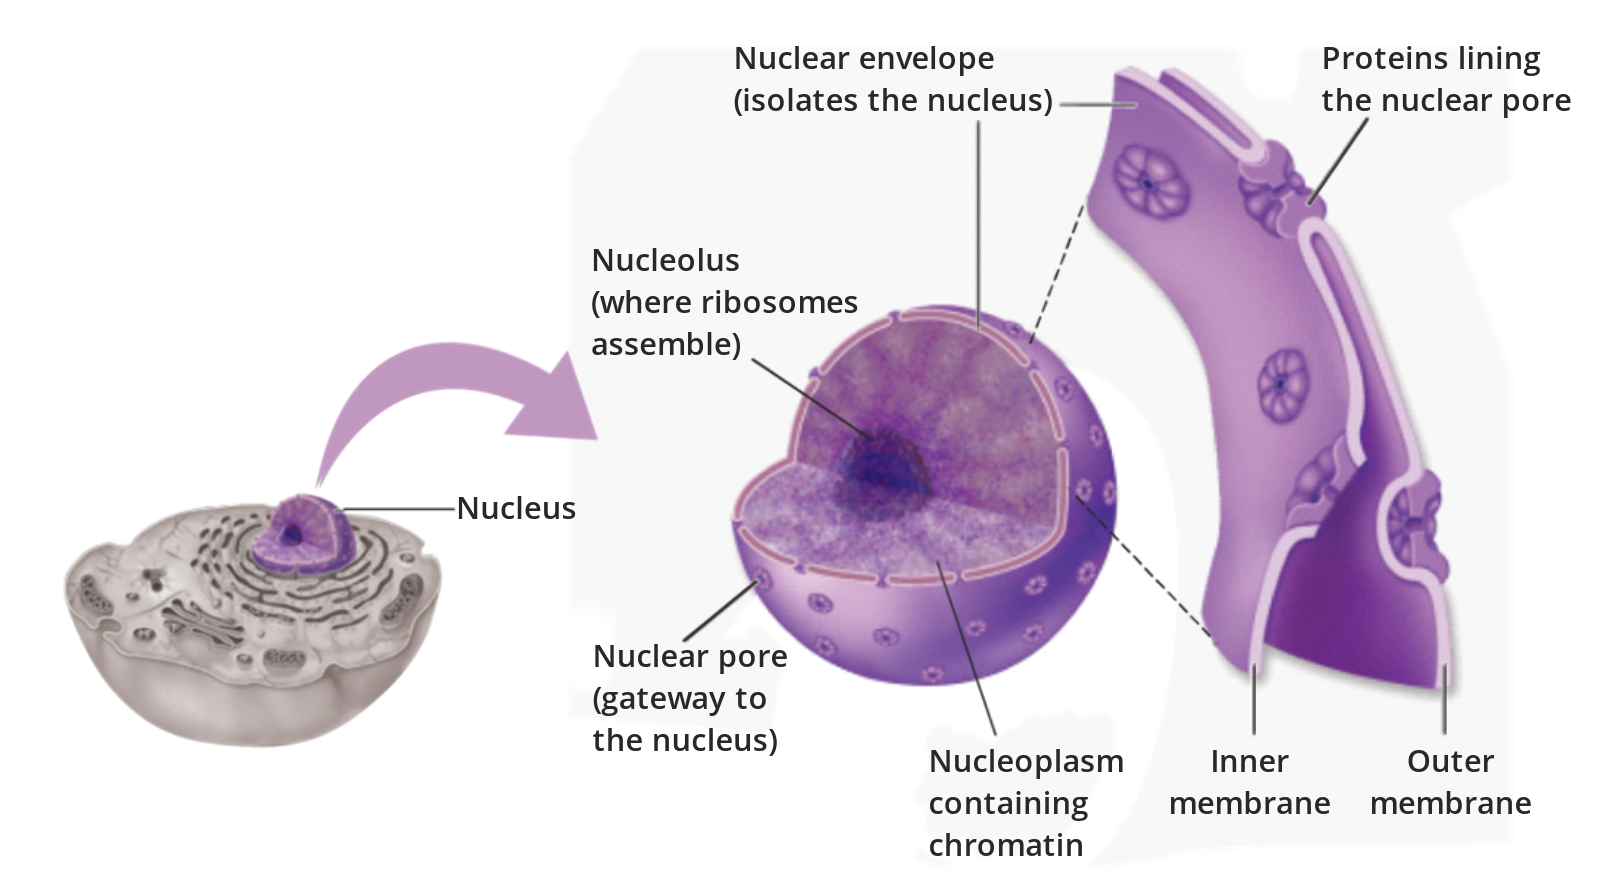
\includegraphics[width = \textwidth]{nucleus-structure}\]

\subsection{Cytoskeleton}
\label{sec:orga8f952c}
\[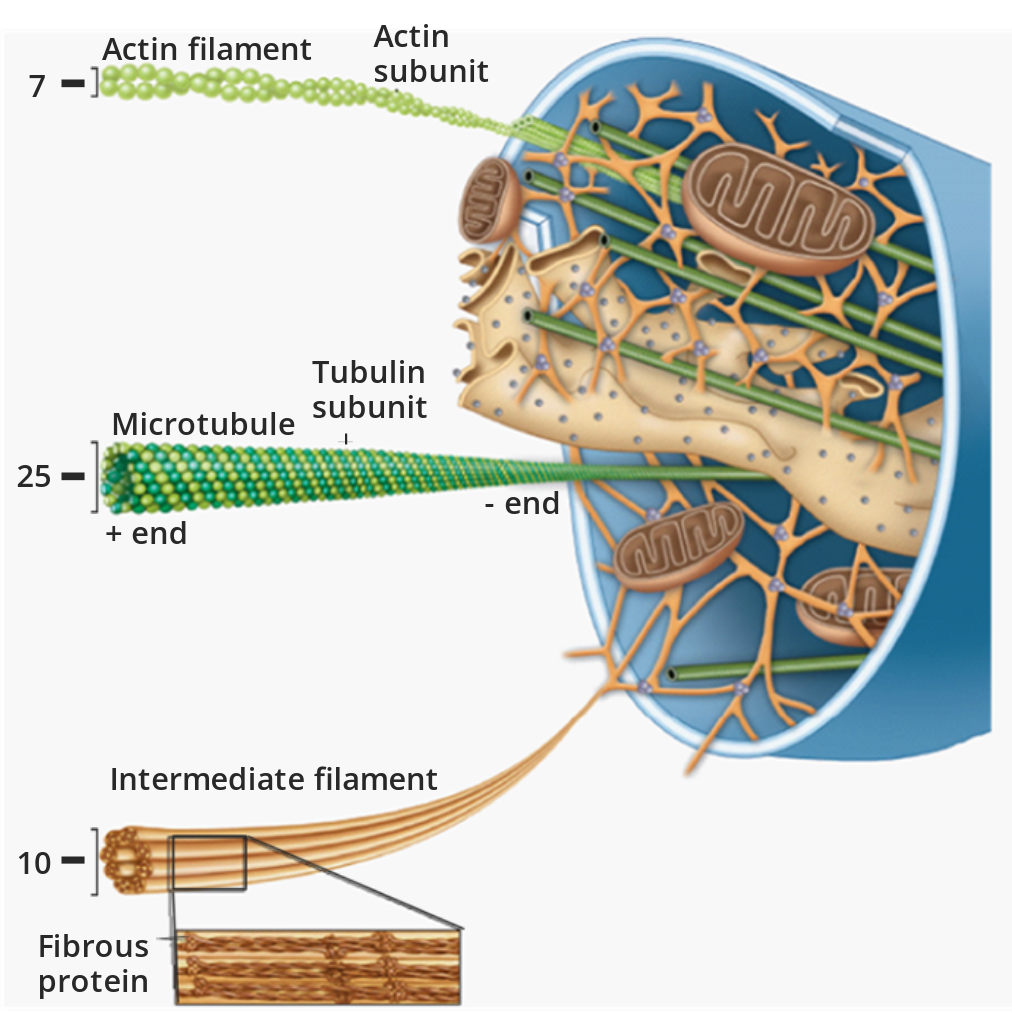
\includegraphics[width = \textwidth]{cytoskeleton-structure}\]

\subsection{Centrioles}
\label{sec:org423367e}
\[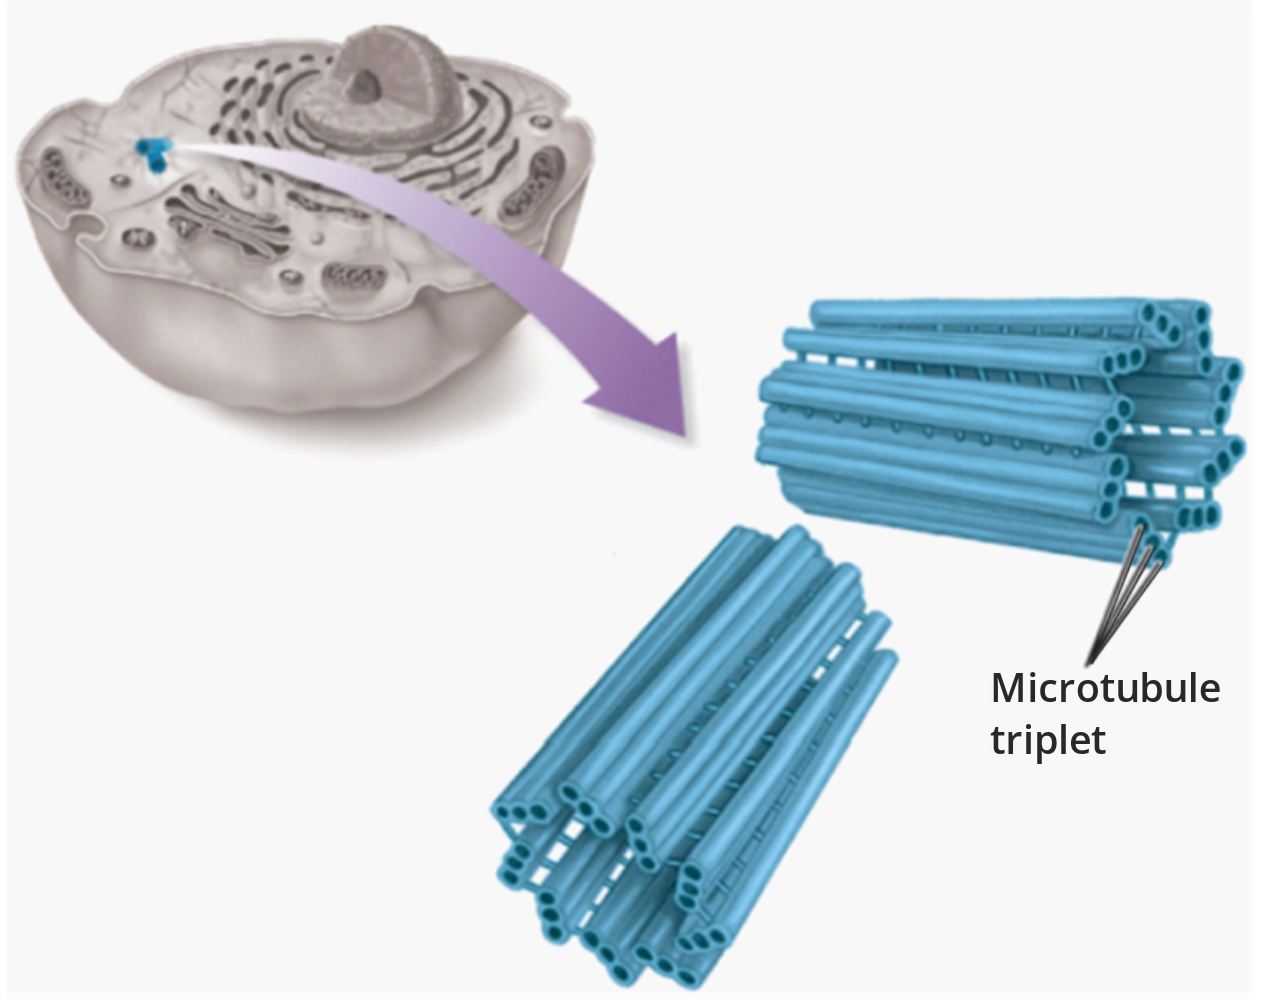
\includegraphics[width = \textwidth]{centrioles-structure}\]

\subsection{Flagella and Cilia}
\label{sec:org967abc8}
\[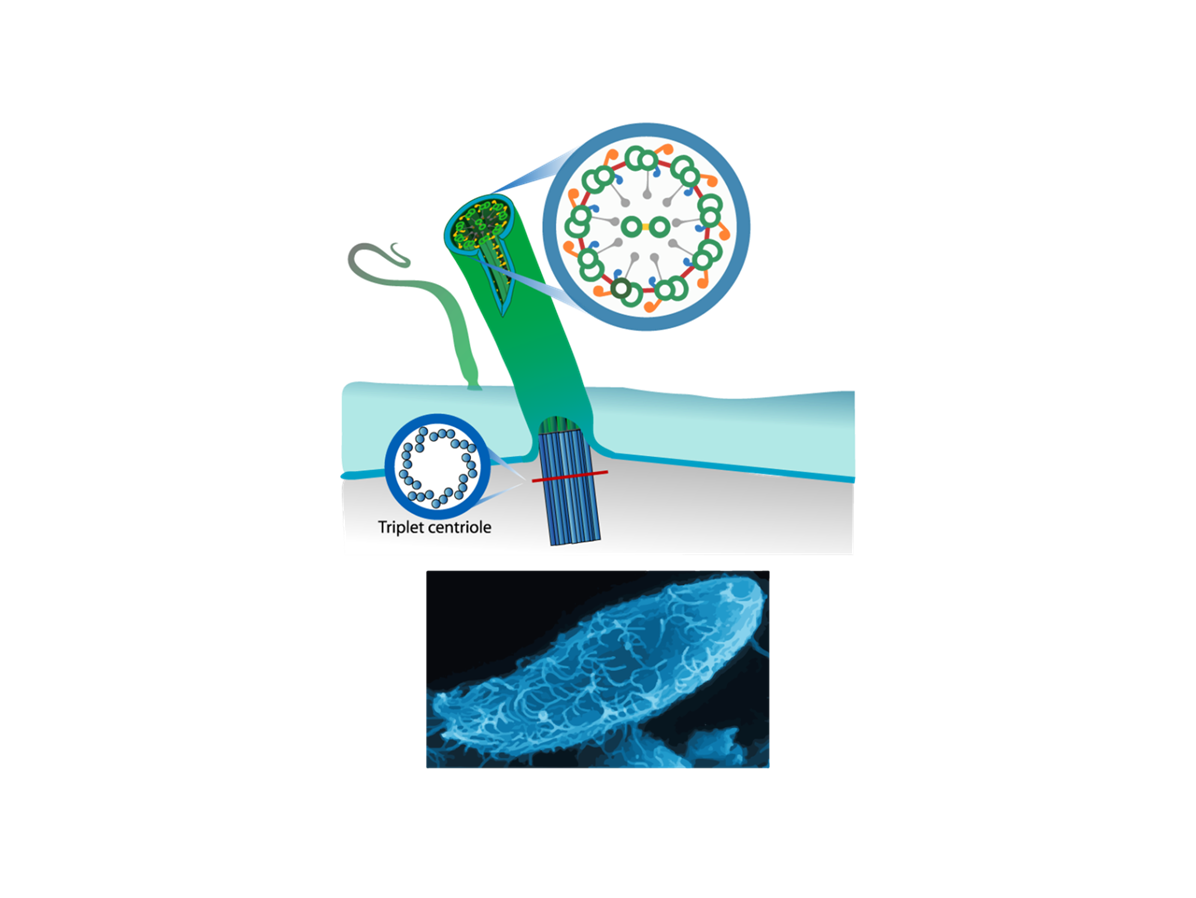
\includegraphics[width = \textwidth]{flagella-and-cilia-structure}\]
\end{document}